%  LaTeX support: latex@mdpi.com 
%  For support, please attach all files needed for compiling as well as the log file, and specify your operating system, LaTeX version, and LaTeX editor.

%=================================================================
\documentclass[mathematics,article,submit,pdftex,moreauthors]{Definitions/mdpi} 
% For posting an early version of this manuscript as a preprint, you may use "preprints" as the journal and change "submit" to "accept". The document class line would be, e.g., \documentclass[preprints,article,accept,moreauthors,pdftex]{mdpi}. This is especially recommended for submission to arXiv, where line numbers should be removed before posting. For preprints.org, the editorial staff will make this change immediately prior to posting.

%--------------------
% Class Options:
%--------------------
%----------
% journal
%----------
% Choose between the following MDPI journals:
% acoustics, actuators, addictions, admsci, adolescents, aerospace, agriculture, agriengineering, agronomy, ai, algorithms, allergies, alloys, analytica, animals, antibiotics, antibodies, antioxidants, applbiosci, appliedchem, appliedmath, applmech, applmicrobiol, applnano, applsci, aquacj, architecture, arts, asc, asi, astronomy, atmosphere, atoms, audiolres, automation, axioms, bacteria, batteries, bdcc, behavsci, beverages, biochem, bioengineering, biologics, biology, biomass, biomechanics, biomed, biomedicines, biomedinformatics, biomimetics, biomolecules, biophysica, biosensors, biotech, birds, bloods, blsf, brainsci, breath, buildings, businesses, cancers, carbon, cardiogenetics, catalysts, cells, ceramics, challenges, chemengineering, chemistry, chemosensors, chemproc, children, chips, cimb, civileng, cleantechnol, climate, clinpract, clockssleep, cmd, coasts, coatings, colloids, colorants, commodities, compounds, computation, computers, condensedmatter, conservation, constrmater, cosmetics, covid, crops, cryptography, crystals, csmf, ctn, curroncol, currophthalmol, cyber, dairy, data, dentistry, dermato, dermatopathology, designs, diabetology, diagnostics, dietetics, digital, disabilities, diseases, diversity, dna, drones, dynamics, earth, ebj, ecologies, econometrics, economies, education, ejihpe, electricity, electrochem, electronicmat, electronics, encyclopedia, endocrines, energies, eng, engproc, ent, entomology, entropy, environments, environsciproc, epidemiologia, epigenomes, est, fermentation, fibers, fintech, fire, fishes, fluids, foods, forecasting, forensicsci, forests, foundations, fractalfract, fuels, futureinternet, futureparasites, futurepharmacol, futurephys, futuretransp, galaxies, games, gases, gastroent, gastrointestdisord, gels, genealogy, genes, geographies, geohazards, geomatics, geosciences, geotechnics, geriatrics, hazardousmatters, healthcare, hearts, hemato, heritage, highthroughput, histories, horticulturae, humanities, humans, hydrobiology, hydrogen, hydrology, hygiene, idr, ijerph, ijfs, ijgi, ijms, ijns, ijtm, ijtpp, immuno, informatics, information, infrastructures, inorganics, insects, instruments, inventions, iot, j, jal, jcdd, jcm, jcp, jcs, jdb, jeta, jfb, jfmk, jimaging, jintelligence, jlpea, jmmp, jmp, jmse, jne, jnt, jof, joitmc, jor, journalmedia, jox, jpm, jrfm, jsan, jtaer, jzbg, kidney, kidneydial, knowledge, land, languages, laws, life, liquids, literature, livers, logics, logistics, lubricants, lymphatics, machines, macromol, magnetism, magnetochemistry, make, marinedrugs, materials, materproc, mathematics, mca, measurements, medicina, medicines, medsci, membranes, merits, metabolites, metals, meteorology, methane, metrology, micro, microarrays, microbiolres, micromachines, microorganisms, microplastics, minerals, mining, modelling, molbank, molecules, mps, msf, mti, muscles, nanoenergyadv, nanomanufacturing, nanomaterials, ncrna, network, neuroglia, neurolint, neurosci, nitrogen, notspecified, nri, nursrep, nutraceuticals, nutrients, obesities, oceans, ohbm, onco, oncopathology, optics, oral, organics, organoids, osteology, oxygen, parasites, parasitologia, particles, pathogens, pathophysiology, pediatrrep, pharmaceuticals, pharmaceutics, pharmacoepidemiology, pharmacy, philosophies, photochem, photonics, phycology, physchem, physics, physiologia, plants, plasma, pollutants, polymers, polysaccharides, poultry, powders, preprints, proceedings, processes, prosthesis, proteomes, psf, psych, psychiatryint, psychoactives, publications, quantumrep, quaternary, qubs, radiation, reactions, recycling, regeneration, religions, remotesensing, reports, reprodmed, resources, rheumato, risks, robotics, ruminants, safety, sci, scipharm, seeds, sensors, separations, sexes, signals, sinusitis, skins, smartcities, sna, societies, socsci, software, soilsystems, solar, solids, sports, standards, stats, stresses, surfaces, surgeries, suschem, sustainability, symmetry, synbio, systems, taxonomy, technologies, telecom, test, textiles, thalassrep, thermo, tomography, tourismhosp, toxics, toxins, transplantology, transportation, traumacare, traumas, tropicalmed, universe, urbansci, uro, vaccines, vehicles, venereology, vetsci, vibration, viruses, vision, waste, water, wem, wevj, wind, women, world, youth, zoonoticdis 

%---------
% article
%---------
% The default type of manuscript is "article", but can be replaced by: 
% abstract, addendum, article, book, bookreview, briefreport, casereport, comment, commentary, communication, conferenceproceedings, correction, conferencereport, entry, expressionofconcern, extendedabstract, datadescriptor, editorial, essay, erratum, hypothesis, interestingimage, obituary, opinion, projectreport, reply, retraction, review, perspective, protocol, shortnote, studyprotocol, systematicreview, supfile, technicalnote, viewpoint, guidelines, registeredreport, tutorial
% supfile = supplementary materials

%----------
% submit
%----------
% The class option "submit" will be changed to "accept" by the Editorial Office when the paper is accepted. This will only make changes to the frontpage (e.g., the logo of the journal will get visible), the headings, and the copyright information. Also, line numbering will be removed. Journal info and pagination for accepted papers will also be assigned by the Editorial Office.

%------------------
% moreauthors
%------------------
% If there is only one author the class option oneauthor should be used. Otherwise use the class option moreauthors.

%---------
% pdftex
%---------
% The option pdftex is for use with pdfLaTeX. If eps figures are used, remove the option pdftex and use LaTeX and dvi2pdf.

%=================================================================
% MDPI internal commands
\firstpage{1} 
\makeatletter 
\setcounter{page}{\@firstpage} 
\makeatother
\pubvolume{1}
\issuenum{1}
\articlenumber{0}
\pubyear{2022}
\copyrightyear{2022}
%\externaleditor{Academic Editor: Firstname Lastname}
\datereceived{} 
%\daterevised{} % Only for the journal Acoustics
\dateaccepted{} 
\datepublished{} 
%\datecorrected{} % Corrected papers include a "Corrected: XXX" date in the original paper.
%\dateretracted{} % Corrected papers include a "Retracted: XXX" date in the original paper.
\hreflink{https://doi.org/} % If needed use \linebreak
%\doinum{}
%------------------------------------------------------------------
% The following line should be uncommented if the LaTeX file is uploaded to arXiv.org
%\pdfoutput=1

%=================================================================
% Add packages and commands here. The following packages are loaded in our class file: fontenc, inputenc, calc, indentfirst, fancyhdr, graphicx, epstopdf, lastpage, ifthen, lineno, float, amsmath, setspace, enumitem, mathpazo, booktabs, titlesec, etoolbox, tabto, xcolor, soul, multirow, microtype, tikz, totcount, changepage, attrib, upgreek, cleveref, amsthm, hyphenat, natbib, hyperref, footmisc, url, geometry, newfloat, caption

%%% ДЛЯ РУССКОГО ТЕКСТА закомментировать потом!
%\usepackage{inputenc}
%\usepackage[T2A,T1]{fontenc}
%\usepackage[english,russian]{babel}
%\usepackage{cmap}
%%%


%=================================================================
%% Please use the following mathematics environments: Theorem, Lemma, Corollary, Proposition, Characterization, Property, Problem, Example, ExamplesandDefinitions, Hypothesis, Remark, Definition, Notation, Assumption
%% For proofs, please use the proof environment (the amsthm package is loaded by the MDPI class).

%=================================================================
% Full title of the paper (Capitalized)
\Title{On Solving the Problem of Finding Kinetic Parameters of Catalytic Isomerization of the Pentane-Hexane Fraction Using Parallel Global Search Algorithm}
% Дежурное название: Использование ...алгоритма для определения кинетических параметров процесса каталитической изомеризации пентан-гексановой фракции
% Еще один вариант: О решении задачи определения Kinetic Parameters of Catalytic Isomerization of the Pentane-Hexane Fraction с помощью Parallel Global Search Algorithm
% На английском: On Solving the Problem of Finding Kinetic Parameters of Catalytic Isomerization of the Pentane-Hexane Fraction Using Parallel Global Search Algorithm



% MDPI internal command: Title for citation in the left column
\TitleCitation{On Solving the Problem of Finding Kinetic Parameters}

% Author Orchid ID: enter ID or remove command
\newcommand{\orcidauthorA}{0000-0001-5273-2471} % Add \orcidA{} behind the author's name
\newcommand{\orcidauthorB}{0000-0001-6776-0096}
\newcommand{\orcidauthorC}{0000-0002-8736-0652} % Add \orcidB{} behind the author's name
\newcommand{\orcidauthorD}{0000-0001-6073-9585} 
\newcommand{\orcidauthorE}{0000-0003-4219-4870} 

% Authors, for the paper (add full first names)
\Author{Konstantin Barkalov $^{1}$\orcidA{}, Irek Gubaydullin $^{2,3}$, Evgeny Kozinov$^{1}$\orcidB{}, Ilya Lebedev $^{1}$\orcidC{}, Roza Faskhutdinova\orcidD{} $^{2,3}$, Azamat Faskhutdinov$^{2}$ and Leniza Enikeeva $^{3,4,}$*\orcidE{}}

%\longauthorlist{yes}

% MDPI internal command: Authors, for metadata in PDF
\AuthorNames{Konstantin Barkalov, Irek Gubaydullin, Evgeny Kozinov, Ilya Lebedev, Roza Faskhutdinova, Azamat Faskhutdinov, Leniza Enikeeva}

% MDPI internal command: Authors, for citation in the left column
\AuthorCitation{Barkalov, B.; Gubaydullin, I.; Kozinov, E.; Lebedev, I.; Faskhutdinova, R.; Faskhutdinov, A.; Enikeeva, L.}
% If this is a Chicago style journal: Lastname, Firstname, Firstname Lastname, and Firstname Lastname.

\address{%
$^{1}$ \quad Lobachevsky State University of Nizhny Novgorod, Nizhny Novgorod, Russia; konstantin.barkalov@itmm.unn.ru\\
$^{2}$ \quad Institute of Petrochemistry and Catalysis – Subdivision of the Ufa Federal Research Centre of RAS, Ufa, Russia; irekmars@mail.ru \\
$^{3}$ \quad Ufa State Petroleum Technological University, Ufa, Russia; roza\_fask@mail.ru\\
$^{4}$ \quad Novosibirsk State University, Novosibirsk, Russia; leniza.enikeeva@yandex.ru
}

% Contact information of the corresponding author
\corres{Correspondence: leniza.enikeeva@yandex.ru (E.L.); konstantin.barkalov@itmm.unn.ru (B.K.) }

% Current address and/or shared authorship
%\firstnote{Current address: Affiliation 3.} 
%\secondnote{These authors contributed equally to this work.}
% The commands \thirdnote{} till \eighthnote{} are available for further notes

%\simplesumm{} % Simple summary

%\conference{} % An extended version of a conference paper

% Abstract (Do not insert blank lines, i.e. \\) 
\abstract{The article is devoted to the problem of developing a kinetic model of a complex chemical reaction using a parallel optimization method. The design of the kinetic model consists in finding the kinetic parameters of the reaction, which cannot be calculated analytically, and since the chemical reaction involves many stages, the optimization problem is multi-extreme. As a chemical reaction, the process of catalytic isomerization of the pentane-hexane fraction is considered, which is now important due to the switch of the oil refining industry to the production of gasoline corresponding to the Euro-5 standard. To solve the optimization problem, the authors have developed parallel global search algorithm and a program based on Lipschitz optimization. The kinetic parameters found made it possible to develop a mathematical model of the process, which gives good agreement with industrial data.}

% Keywords
\keyword{kinetic model; inverse problems of chemical kinetics; mathematical modeling; catalytic isomerisation of pentane-hexane fraction; Lipschitz optimization; black-box functions; parallel computing} 


% The fields PACS, MSC, and JEL may be left empty or commented out if not applicable
%\PACS{J0101}
%\MSC{}
%\JEL{}

%%%%%%%%%%%%%%%%%%%%%%%%%%%%%%%%%%%%%%%%%%
% Only for the journal Diversity
%\LSID{\url{http://}}

%%%%%%%%%%%%%%%%%%%%%%%%%%%%%%%%%%%%%%%%%%
% Only for the journal Applied Sciences
%\featuredapplication{Authors are encouraged to provide a concise description of the specific application or a potential application of the work. This section is not mandatory.}
%%%%%%%%%%%%%%%%%%%%%%%%%%%%%%%%%%%%%%%%%%

%%%%%%%%%%%%%%%%%%%%%%%%%%%%%%%%%%%%%%%%%%
% Only for the journal Data
%\dataset{DOI number or link to the deposited data set if the data set is published separately. If the data set shall be published as a supplement to this paper, this field will be filled by the journal editors. In this case, please submit the data set as a supplement.}
%\datasetlicense{License under which the data set is made available (CC0, CC-BY, CC-BY-SA, CC-BY-NC, etc.)}

%%%%%%%%%%%%%%%%%%%%%%%%%%%%%%%%%%%%%%%%%%
% Only for the journal Toxins
%\keycontribution{The breakthroughs or highlights of the manuscript. Authors can write one or two sentences to describe the most important part of the paper.}

%%%%%%%%%%%%%%%%%%%%%%%%%%%%%%%%%%%%%%%%%%
% Only for the journal Encyclopedia
%\encyclopediadef{For entry manuscripts only: please provide a brief overview of the entry title instead of an abstract.}

%%%%%%%%%%%%%%%%%%%%%%%%%%%%%%%%%%%%%%%%%%
\begin{document}

%%%%%%%%%%%%%%%%%%%%%%%%%%%%%%%%%%%%%%%%%%
\section{Introduction}

Due to the transition of the domestic oil refining industry to the production of gasoline conforming to the Euro-5 standard, an urgent task is to reduce the content of aromatic hydrocarbons and, in particular, benzene in motor fuel while maintaining the octane value. In connection with the transition of the oil refining industry to the production of motor gasoline conforming to Euro-5 and Euro-6 standards, the reduction of aromatic hydrocarbons in motor fuel and, mainly, benzene becomes an urgent task. At the same time, removing aromatic hydrocarbons, which are high-octane components, it is necessary to preserve the octane number of gasoline. It is known that hydrocarbons of branched structure have a higher octane number than hydrocarbons of linear structure. For example, in $n$-pentane, the octane number according to the research method is 62 points, and in $iso$-pentane it is 93 points. On an industrial scale, catalytic isomerization units of light paraffins have been introduced to produce hydrocarbons of an isomeric structure. The catalytic isomerization of light paraffins, in turn, makes it possible to obtain a high-octane component of automobile gasoline with a minimum content of aromatic hydrocarbons. The main advantage of this process is the production of high-octane gasoline, while aromatic hydrocarbons are practically not formed. Straight-run gasoline fractions with boiling limits of 62-70 $^0$C containing mainly $n$-pentane and $n$-hexane, pentane-hexane fractions from gas condensate or from gas fractionation plants, as well as catalytic reforming raffinates are used as feedstock for catalytic isomerization. Modern bifunctional catalysts are used to carry out the process. In order to prevent coke deposition, the catalytic isomerization process is carried out in a hydrogen-containing gas environment under pressure.

Computer information technologies are widely used in the modeling of production processes and today it is difficult to imagine research activities without the use of modern means of constructing and using models. Moreover, special attention is currently being paid to the development of a detailed kinetic model of complex industrial processes. Based on these models, it is possible to significantly increase the efficiency of the process, while minimally spending energy and material resources. The main advantage of such methods is the absence of additional costs for the construction of pilot plants. The developed model should describe the process within a wide range of operating conditions, have high flexibility, allowing for changes, calculations of the composition of the reaction mixture, etc.

In the article \cite{enik2021} we have already reviewed this process, but in order to simplify the model, the scheme of chemical transformations, in particular hydrocracking reactions, have been revised. Thus, the most probable hydrocracking reactions based on the carbonium-ion mechanism were formed. The new transformation scheme implies the recalculation of the kinetic parameters of the reaction, which form a mathematical model of the process.

In the article \cite{enik2021}, a genetic algorithm was used to calculate kinetic parameters, and the calculation time of kinetic parameters was about 10 hours. Therefore, in order to develop a mathematical model of a new transformation scheme, the question of choosing a more effective optimization method arises.

In the complex problems of chemical kinetics, kinetic constants of reactions cannot be found analytically, they can only be found using numerical methods (see, for example, \cite{Zaynullin2020,Enikeeva2020,Koledina2019}). In this case, the quality criterion (objective function) is set in the form of a certain algorithm, which includes the stage of numerical modeling, which, in turn, makes it compute-intensive. Furthermore, in the inverse problems of chemical kinetics, the objective function can be substantially multiextremal, i.e., having many local extremes along the global one. 

Computational algorithms for solving such multiextremal problems (global optimization methods) differ vastly from local optimization techniques since they require the study of the entire search domain (see, for example, \cite{PaulaviciusZilinskas2014,Sergeyev2017}). These methods can be divided into two classes: metaheuristic and deterministic. Metaheuristic algorithms are usually based on simulations of processes occurring in the wild.
Examples of metaheuristic algorithms are simulated annealing, evolutionary computing, etc. (see, for example, \cite{Battiti2009,Eiben2015}).
These algorithms are included in many software libraries for solving global optimization problems (for example, MATLAB Global Optimization Toolbox, Scipy.Optimize, etc.).
Due to the operation speed and low requirements for computing resources (in particular, memory), metaheuristic algorithms have become widespread for solving practical problems. However, the solution to the problem found by such an algorithm is, in general, local and can be located far from the global optimum \cite{Kvasov2018}. 

It is also possible to construct deterministic methods of global search, which are different from brute force algorithms and metaheuristic algorithms. Such methods are associated with the presence and consideration of a priori assumptions about the problem properties. 
One of the natural assumptions about the problem is that changing the values of an objective function is limited by changes of its argument. In this case, the function satisfies the Lipschitz condition, and the problem itself is called the Lipschitz global optimization problem. The central direction of the development of modern methods of Lipschitz optimization is the development of parallel algorithms. It is assumed that the values of the objective function are determined as a result of solving some other task and require a costly computational experiment.


This paper reflects the results of applying parallel methods of Lipschitz optimization developed in \cite{Barkalov2016,Strongin2018,Sysoyev2017}, to the solution of inverse problems of chemical kinetics.  
The main part of the paper is structured as follows. 

Section \ref{sec_matmodel} provides a description of the mathematical model of the chemical reaction under study. Section \ref{sec_GSA} discusses the standard formulation of the Lipschitz global optimization problem and the algorithm for solving it. Section \ref{sec_numexper} outlines the issues related to the technical aspects of the implementation of the parallel algorithm. The physico-chemical interpretation of the results of numerical calculations using the developed parallel algorithm is presented in the Section \ref{sec_discussion}. 
%The last section contains the conclusion and plans for future work.

\section{Mathematical model}\label{sec_matmodel}

Let's consider the mechanism of chemical transformations of the isomerization of the pentane-hexane fraction. The reaction consists of 48 reaction stages, which are presented in the table \ref{tab_chemistry}. The following abbreviations were adopted: 2-MP is 2-methylpentane; 3-MP is 3-methylpentane; 2,2-DMB is 2,2-dimethylbutane; 2,3-DMB is 2,3-dimethylbutane; CH* is cyclohexane; MCP is methyl cyclopentane; B is benzene; CP is cyclopentane.

\begin{table}[H] 
\caption{Chemical transformations of the catalytic isomerization of the pentane-hexane fraction.\label{tab_chemistry}}
\newcolumntype{C}{>{\centering\arraybackslash}X}
\begin{tabularx}{\textwidth}{CC}
\toprule
 \textbf{Reaction stages} & \textbf{Reaction stages} \\
\midrule
1) $n$-C$_5$H$_{12}$ $\rightarrow$ $iso$-C$_5$H$_{12}$ & 25) $n$-C$_6$H$_{14}$ $\rightarrow$ CH* + H$_2$\\
2) $iso$-C$_5$H$_{12}$ $\rightarrow$ $n$-C$_5$H$_{12}$ & 26) CH* + H$_2$ $\rightarrow$ $n$-C$_6$H$_{14}$ \\
3) $n$-C$_6$H$_{14}$ $\rightarrow$ 2-MP & 27) 2-MP $\rightarrow$ MCP+ H$_2$ \\
4) 2-MP $\rightarrow$ $n$-C$_6$H$_{14}$ & 28) MCP + H$_2$ $\rightarrow$ 2-MP  \\
5) $n$-C$_6$H$_{14}$ $\rightarrow$ 3-MP & 29) 3-MP $\rightarrow$ MCP + H$_2$ \\
6) 3-MP $\rightarrow$ $n$-C$_6$H$_{14}$  & 30) MCP + H$_2$ $\rightarrow$ 3-MP \\
7)  2-MP $\rightarrow$ 3-MP & 31) 2,2-DMB $\rightarrow$ MCP + H$_2$ \\
8) 3-MP $\rightarrow$ 2-MP  & 32) MCP + H$_2$ $\rightarrow$ 2,2-DMB \\
9) 2-MP $\rightarrow$ 2,2-DMB  & 33) 2,3-DMB $\rightarrow$ MCP + H$_2$ \\
10) 2,2-DMB $\rightarrow$ 2-MP  & 34) MCP + H$_2$ $\rightarrow$ 2,3-DMB \\
11) 2-MP $\rightarrow$ 2,3-DMB  & 35) CP + H$_2$ $\rightarrow$ $n$-C$_5$H$_{12}$ \\
12) 2,3-DMB $\rightarrow$ 2-MP  & 36) $n$-C$_5$H$_{12}$ $\rightarrow$ CP + H$_2$ \\
13) 3-MP $\rightarrow$ 2,2-DMB  & 37) $n$-C$_4$H$_{10}$ $\rightarrow$ $iso$-C$_4$H$_{10}$ \\
14) 2,2-DMB $\rightarrow$ 3-MP  & 38) $iso$-C$_4$H$_{10}$ $\rightarrow$ $n$-C$_4$H$_{10}$ \\
15) 3-MP $\rightarrow$ 2,3-DMB  & 39) $n$-C$_5$H$_{12}$ + H$_2$ $\rightarrow$ C$_3$H$_8$ + C$_2$H$_6$ \\
16) 2,3-DMB $\rightarrow$ 3-MP  & 40) $n$-C$_5$H$_{12}$ + H$_2$ $\rightarrow$ $n$-C$_4$H$_{10}$ + CH$_4$ \\
17) 2,2-DMB $\rightarrow$ 2,3-DMB  & 41) $iso$-C$_5$H$_{12}$ + H$_2$ $\rightarrow$ $iso$-C$_4$H$_{10}$ + CH$_4$ \\
18) 2,3-DMB $\rightarrow$ 2,2-DMB & 42) $n$-C$_6$H$_{14}$ + H$_2$ $\rightarrow$ 2C$_3$H$_8$ \\
19) B + 3H$_2$ $\rightarrow$ CH*  & 43) $n$-C$_6$H$_{14}$ + H$_2$ $\rightarrow$ $n$-C$_5$H$_{12}$ + CH$_4$ \\
20) CH* $\rightarrow$ B + 3H$_2$ & 44) $n$-C$_6$H$_{14}$ + H$_2$ $\rightarrow$ $n$-C$_4$H$_{10}$ + C$_2$H$_6$ \\
21) B + 3H$_2$ $\rightarrow$ MCP  & 45) 2-MP + H$_2$ $\rightarrow$ $iso$-C$4$H$_{10}$ + C$_2$H$_6$ \\
22) MCP $\rightarrow$ B + 3H$_2$  & 46) 3-MP + H$_2$ $\rightarrow$ $iso$-C$_5$H$_{12}$ + CH$_4$ \\
23) CH* $\rightarrow$ MCP & 47) 2,2-DMB + H$_2$ $\rightarrow$ $iso$-C$_5$H$_{12}$ + CH$_4$ \\
24) MCP $\rightarrow$ CH*  & 48) 2,3-DMB + H$_2$ $\rightarrow$ $iso$-C$_5$H$_{12}$ + CH$_4$ \\
\bottomrule
\end{tabularx}
\end{table}

Mathematical model of the chemical process is a non-linear system of differential equations \cite{Koledina2016KineticsAM,enik2021,logan}:
\begin{linenomath}
\begin{equation}\label{eq_concentrations}
\dfrac{dx_i}{d\tau} = \sum_{j=1}^J \nu_{ij} w_j, i = 1,...,I,
\end{equation}
\begin{equation}\label{eq_rate}
w_{j} = k_j \prod_{i=1}^I \left( \dfrac{x_i}{F} \right),
\end{equation}
\begin{equation}\label{eq_constant}
k_j = k^0_j \exp \left( -\dfrac{E_j}{RT} \right)
\end{equation}
\end{linenomath}
with initial values: at $\tau = 0$, $x_i(0) = x_i^0$, where $\nu_{ij}$ are stoichiometric coefficients of stages of chemical reaction; $J$ is number of stages ($J = 48$), $x_i$ is molar flow rate of the $i$-th component of reaction, kmol/h; $I$ is the number of components ($I = 17$); $w_j$ is the rate of the $j$-th stage of reaction, kmol/(h$\cdot$kg cat.), $E_j$ is activation energy of reaction stage, J/mol; $R$ is the universal gas constant ($R$=8,31 J/(mol$\cdot$K), $T$ is temperature, K; $k_j$ are pre-exponentional factors, kmol/(h$\cdot$kg cat.); $\tau$ is conditioned contact time, (kg cat.); $F$ is the total molar flow rate, kmol/h.

The mathematical model involves such parameters as the raw material flow rate $F$ in the reactor and temperature $T$, but these two parameters also depend on $\tau$, therefore it is necessary to write equations on them, because technological process is non-isothermal:
\begin{linenomath}
\begin{equation}\label{eq_temper}
\dfrac{dT}{d\tau} = \dfrac{\sum_{i=1}^I\left( \dfrac{dx_i}{d\tau} \cdot \Delta H^i_{f,T} \right) }{\sum_i^J \left(x_i C^T_{p_i} \right) },
\end{equation}\label{eq_flow}
\begin{equation}
\dfrac{dF}{d\tau} = \sum_{i=1}^I  \dfrac{x_i}{d\tau}
\end{equation}
\end{linenomath}
with initial condition: at $\tau = 0$, $T(0) = T^0$, where $T$ is temperature, K, $\Delta H^i_{f,T}$ is enthalpy of the $i$-th component formation at temperature $T$, J/mol, $C^T_{p_i}$ is specific heat capacity of the $i$-th component at temperature $T$, (J/mol$\cdot$K), $F$ is mole discharge of the flow, kmol/h.

Thus, when solving the inverse kinetic problem, the direct problem is repeatedly solved, which includes the numerical integration of equations \eqref{eq_concentrations}, \eqref{eq_temper} and \eqref{eq_flow}. After finding the numerical values of the molar flow rate $x_i$, temperature $T$ and total molar flow rate $F$, these values are compared with the corresponding industrial data obtained during the three days of operation of the catalytic isomerization unit \cite{enik2021}, which is a minimization task:

\begin{linenomath}
\begin{equation}
FF = \dfrac{\sum_{i=1}^I \left| \dfrac{y_i^{exp} - y_i^{calc}}{y_i^{exp}} \right|}{I} \rightarrow \min,
\end{equation}
\end{linenomath}

where I is the number of observed parameters (I=19, of which 17 parameters are $x_i$, one parameter is $T$ and one parameter is $F$),  $y_{i}^{exp}$ are industrual data, $y_{i}^{calc}$ are numerical values of concentrations of reaction substances obtained by solving a direct kinetic problem. As a result of solving the inverse problem, the kinetic parameters $k^0_j$ and $E_j$ included in the Arrhenius equation \eqref{eq_rate} will be obtained. Since the number of reaction stages is 48, the kinetic model will contain 96 kinetic parameters (activation energy $E_j$ and pre-exponential multiplier $k^0_j$ for each stage), however, the authors decided to fix some of the parameters as already known for chemical reasons, so the number of optimized parameters was reduced to 24.

\section{Parallel Algorithm for Solving Global Optimization Problems }\label{sec_GSA}

\subsection{Statement of the global optimization problem}

As stated above, from a mathematical point of view, the inverse problem of chemical kinetics can be considered a Lipschitz global optimization problem. 
In general, the problem of the specified class can be formulated as follows:
\begin{gather}
 \phi^* = \phi(y^\ast)=\min{\left\{\phi(y):y\in D\right\}}, \label{problemN}\\
 D=\left\{y\in R^N: a_i\leq y_i \leq b_i, \;  1\leq i \leq N\right\} \label{D},
\end{gather}
where $a,b \in R^N$ are boundaries of the search domain, and the objective function $\phi(y)$ satisfies the Lipschitz condition
\begin{equation}\label{Lip}
\left|\phi(y_1)-\phi(y_2)\right|\leq L\left\|y_1-y_2\right\|,\; y_1,y_2 \in D.
\end{equation}

The criterion $\phi(y)$ is assumed to be multiextremal and is given in the form of some computational algorithm. The input of this algorithm is supplied with a parameter vector, and the output is the corresponding function value. Such functions are often referred to as ``black-box'' functions. It is also assumed that each calculation of the function value at the search domain point (hereinafter also referred to as trial) is a laborious operation and requires significant computational resources. As noted in the introduction, this statement of the problem fully corresponds to the inverse problem of chemical kinetics.

The Lipschitz condition (\ref{Lip}) can be used to construct estimates of the function global minimum, which can serve as a foundation for designing global optimization algorithms and proving their convergence conditions (see, for example, \cite{Strongin2000}).

One of the main difficulties in solving Lipschitz global optimization problems is the so-called ``curse of dimensionality'' --- the exponential increase in the number of trials required to solve a problem with a given accuracy, accompanied by the increasing dimensionality of the problem. It is possible to smooth this effect while maintaining the accuracy of the solution by constructing significantly uneven coverages of the search domain with trial points.

Known examples of such methods are DIvide RECTangles (DIRECT) algorithm \cite{Jones1993}, the simplicial partitions algorithm \cite{PaulaviciusZilinskas2014}, the diagonal partitions algorithm \cite{Sergeyev2017}. These techniques are based on adaptive partitioning of the search domain into a finite number of subdomains at each iteration.
Then the need for further subdivision for a more detailed study of these subdomains is estimated (using the accumulated information about the objective function). 
A fundamentally different approach to solving a multidimensional problem (\ref{problemN}) is its reduction to one or more one-dimensional problems followed by the use of efficient methods of one-dimensional optimization. Such reduction may be accomplished, for example, by a recursive optimization scheme \cite{Grishagin2018} or by Peano curves \cite{Barkalov2018}. The latter approach is used in this work.

Using a continuous single-valued correspondence (Peano curve) $y(x)$ of the real axis segment $[0,1]$ onto hyperinterval $D$ from (\ref{D}), a multidimensional problem (\ref{problemN}) can be reduced to a one-dimensional one
\[
\phi(y^\ast)=\phi(y(x^\ast))=\min{\left\{\phi(y(x)): x\in[0,1]\right\}}.
\]
It is known \cite{Strongin2000, Sergeyev2013} that the reduced one-dimensional function $\phi(y(x))$ will no longer be Lipschitzian, but will satisfy the H{\"o}lder condition
\[
\left|\phi(y(x_1))-\phi(y(x_2))\right|\leq H\left|x_1-x_2\right|^{1/N},
\]
where the H{\"o}lder constant $H$ is associated with the Lipschitz constant $L$ by the formula $ H=2 L \sqrt{N+3}$.

Specific methods of numerical construction of this kind of mappings (called evolvents) are discussed in \cite{Strongin2000,Sergeyev2013}.
Here we note that evolvent will approximate the theoretical Peano-Hilbert curve with an accuracy of $2^{-m}$, where $m$ is the parameter that sets the approximation accuracy. Examples of evolvent for different dimensions are shown in Fig.~\ref{fig:Peano}.

\begin{figure}
\center
\begin{minipage}{0.45\linewidth}
\center{\includegraphics[width=0.9\linewidth]{fig1a.JPG} \\ (a)}
\end{minipage}
\begin{minipage}{0.45\linewidth}
\center{\includegraphics[width=0.9\linewidth]{fig1b.JPG} \\ (b)}
\end{minipage}
\caption{Evolvents with $m=4$ and (a) $N=2$, (b) $N=3$.}\label{fig:Peano}
\end{figure}   


Thus, under this approach, the search trial at some point $x^k\in[0,1]$ will consist of constructing the image $y^k=y(x^k)$ first, and only then of calculating the function value $ z^k = \phi(y^k)$.
We will call the three values $\{x^k,y ^k,z^k\}$ the trial result.

\subsection{Asynchronous parallel algorithm used to determine the global minimum of a function}

The parallel algorithm used in this study is based on the information-statistical approach to the development of global optimization methods, the theoretical foundations of which are set out in \cite{Strongin2000}. 

We have implemented an asynchronous paralleling scheme of the ``master/worker'' type. The master process performs a global search algorithm, in which the search information is accumulated. Then the Lipschitz constants for the objective function are estimated on its basis, and the points of new trials are calculated and distributed over the work processes. Worker-processes receive points from the master, carry out new trials in them, and send the results of the trials to the master. 

Let us assume that at each iteration, the master calculates one new trial  point and transfers it for processing to the worker. At the same time, a trial performed by a worker is a much more labor-intensive operation than selection of a new point by a master, which eliminates the worker downtime. 
In this case, the total number of trials performed by each worker  will depend on the labor intensity of the specific trial and cannot be estimated in advance.

When describing a parallel algorithm, let us assume that there is one process master and $p$ workers. The upper index will indicate the serial number of the trial performed, and the lower index will be used to number the trials in ascending order of the coordinate.
 
The initial iteration is carried out according to a special rule. The master process (let us assume that this is the process No 0) initiates  $p$ parallel trials at $p$ different points of the search region, two of which are boundary points, and the rest are arbitrary internal points (for example, uniformly distributed). Thus, the initial trials are carried out at the points $\{y(x^1), y(x^2), ...,y(x^p)\}$, where $x^1 = 0$, $x^p = 1$, $x^i\in(0,1), i=2,..., p-1$.

Let us suppose that the master-process has obtained the results of $k$ trials, and at the current time the worker-processes are conducting trials at the points
$\{y(x^{k+1}), y(x^{k+2}), ...,y(x^{k+p})\}$.

Let one of the processes (without limiting the commonality, we can assume that this is the process No 1), at some point in time complete the trial at the point $y(x^{k+1})$.
The remaining processes are at the stage of conducting their trials, i.e. at these points multiple trials have already initiated, but have not yet been finalized.

Then the No 1 process forwards to the master process the trial results, i.e. the three values $\{x^{k+1},y^{k+1},z^{k+1}\}$.
The master saves the results in its information base and selects a new trial point $x^{k+p+1}$ for the process No 1 in accordance with the rules described below.

Step 1. Renumber he point of the set 
\[
X_k = \left\{x^1, x^2,...,x^{k+p} \right\},
\]
which contains all the points at which the trials either have been carried out or are being carried out by the lower index in ascending order, i.e.
\[
0=x_1<x_2<...<x_{x+p}=1.
\]
Step 2. Calculate values
\[
M_1=\max \left\{ \frac{ \left|z_i - z_{i-1} \right|}{(x_i-x_{i-1})^{1/N}} : x_{i-1} \notin I_k, x_i \notin I_k, 2\leq i\leq k+p \right\},
\]
\[
M_2=\max \left\{ \frac{ \left|z_{i+1} - z_{i-1} \right|}{(x_{i+1}-x_{i-1})^{1/N}} : x_i \in I_k, 2\leq i < k+p \right\},
\]
\[
M=\max\{M_1,M_2\},
\]
where $z_i=\phi(y(x_i))$, if $x_i \notin I_k, \; 1\leq i \leq k+p$.  If the value $M$ is 0, assign $M=1$. The values $z_i=\phi(y(x_i))$ at $x_i \in I_k$ are undefined because the trials at $x_i \in I_k$ are not finished yet.

Step 3. For each interval $(x_{i-1},x_i), \; x_{i-1} \notin I_k, x_i \notin I_k, \; 2\leq i\leq k+p$, calculate the value 
\[
R(i)=rM\Delta_i+\frac{(z_i-z_{i-1})^2}{rM\Delta_i}-2(z_i+z_{i-1}),
\]
called the characteristic of this interval. Here $\Delta_i=\left(x_i-x_{i-1}\right)^{1/N}$, and $r>1$ is the reliability parameter of the method.

Step 4. Select the interval $[x_{t-1},x_t]$ with the highest characteristic value, i.e.
\[
R(t) = \max \left\{ R(i): \; x_{i-1} \notin I_k, x_i \notin I_k, \; 2\leq i\leq k+p \right\}.
\]

Step 5. Calculate the point $x^{k+p+1} \in (x_{t-1},x_t)$ according to the formula
\[
x^{k+p+1} = \frac{x_{t}+x_{t-1}}{2} - \mathrm{sign}(z_{t}-z_{t-1})\frac{1}{2r}\left[\frac{\left|z_{t}-z_{t-1}\right|}{M}\right]^N.
\]

Immediately after calculating the point $x^{k+p+1}$ of the next trial, the master appends it to the set $I_k$ and forwards it to the worker, which starts the trial at this point. 

The master stops the algorithm if either the condition $\Delta_{t}<\varepsilon$ (where $t$ is number of the interval with the maximum characteristic from Step 4) or the condition $k>K_{max}$ (where $k$ is the number of trials performed) is met.
The real number $\varepsilon>0$ and the integer $K_{max} \geq 1$ are the algorithm parameters which correspond to the accuracy of the solution search and the maximum number of trials.

The sequential global search algorithm, on the basis of which the proposed asynchronous algorithm was implemented, allows the following interpretation \cite{Molinaro2001}. Using the points of previously performed trials, it is possible to construct a minorant of the objective function, for which the value $-R(i)$, where $R(i)$ is the value of the characteristic of the interval $(x_{i-1}, x_i)$, will be the value of the minorant at the point of its minimum at the interval $(x_{i-1},x_i), 1\leq i\leq k+p$. In accordance with Step 4 of the algorithm, a new trial is carried out in the interval with the lowest value of the minorant. And in accordance with Step 5, the point of the new trial coincides with the minorant minimum point.

The theory of convergence and various modifications of serial and parallel algorithms are detailed in the monographs \cite{Strongin2000,Sergeyev2017}. 
It should be noted that the asynchronous parallelization scheme described here, in contrast to the synchronous schemes used earlier in solving a number of application problems (see \cite{Kalyulin2017, Modorskii2016}), provides a full load of all the processes involved in solving problems with different labor intensity of trials at different points in the search domain.


\subsection{Features of the software implementation of the parallel algorithm}

\begin{figure}
\center{
\includegraphics[width=0.9\linewidth]{fig2.JPG}}
\caption{Implemented scheme of parallel computations (1 -- link via MPI, 2 -- link via streams).}\label{fig:Impl}
\end{figure}   

In our implementation of the global search algorithm, MPI is used to organize parallel calculations. A process with the rank 0 acts as a master, processes with a rank other than 0 act as calculators (workers), see the description of the algorithm in the previous section.

The principle of process interaction (Figure \ref{fig:Impl}, link 1) is as follows. The first step in the master-process is to select $p$ points for trials. The selected trial points are sent to the calculators and the master enters the stand-by state for receiving messages. Messages from the calculators contain the trial result. The obtained information is used to select the point of the next trial. The new point is sent as a message to the calculator. If the stopping condition is met in the algorithm, instead of the trial point the master sends a shutdown message to the calculator.

Each process that performs the role of a calculator creates an instance of the task when it starts, and then goes into a stand-by mode for messages from the master-process. When a message containing a trial point is received, a computational experiment is performed. The results of the experiment are sent to the master. After the experiment, the process itself continues to wait for new messages. When a shutdown message is received, the resources used by the task are released and the main process is terminated.

When implementing the asynchronous scheme, we assumed that the start time of calculating the objective function values is different for each particular process. Our implementation takes into account the fact that the trial point as well as the calculation results represent a small amount of data that can be sent relatively quickly over the network. As a result, basic point-to-point MPI message forwarding operations were used to interact between the master and the calculators (Figure \ref{fig:Impl}, link 1). 

When conducting computational experiments (see next section), the solution of the direct problem of chemical kinetics was performed using MATLAB. In the initial version of the problem, each set of parameters required starting the MATLAB process, transferring the trial point, as well as obtaining the results of computational experiments. A number of additional settings have been made to reduce computing overhead. First, the source code for the computational experiment was compiled into an executable application. Second, the approach in which MATLAB receives a trial point through input stream, and returns the results of computational experiment through output stream was implemented. This approach allowed each calculator to run a process with compiled MATLAB code once, intercept input and output streams, and then perform calculations without waiting for new processes to start. 

\section{Numerical Experiments}\label{sec_numexper}

The asynchronous parallel global search algorithm was implemented on C++; the software was built on Intel MPI and Intel C++ compiler, version 2017.0.1. The objective function of the problem to be solved was implemented in MATLAB 2019b.
In order to check the stability of the developed parallel program, it was launched on three different supercomputers: Lomonosov-2 (Moscow State University), Lobachevsky (University of Nizhni Novgorod), and MVS-10P (Joint Supercomputer Center of the RAS). The main part of the experiments was carried out on the Lomonosov-2 supercomputer with the following computer nodes characteristics: Intel Haswell-EP E5-2697v3 CPU (processor frequency 2.6 GHz, 14 cores), 64 GB of RAM, CentOS 7 operating system.

To solve the optimization problem, a combination of the parallel global search algorithm and a local optimization method was used. In the first stage of the search, the parallel asynchronous algorithm described in Section \ref{sec_GSA} was used. 101 processes were involved in the launch, of which one process was a master and the remaining 100 were workers (calculators). The values of the method parameters were set as follows: the maximum number of trials $K_{max}=3000$, the search accuracy $\varepsilon=10^{-3}$, the reliability parameter $r=3$, the evolvent accuracy parameter $m=12$. At the second stage, the solution was refined using the pattern search method with an accuracy of $\varepsilon=10^{-4}$ and a limit on the number of trials $K_{max}=500$.
The total time for solving the problem was 8109 seconds, an optimum point was found with the objective function value $\phi^* = 0.002115$. Thus, using the developed algorithm, the inverse problem of chemical kinetics was solved and the kinetic parameters of the reaction were found, which are given in the table \ref{tab_kinetics}. 

%%%%%%%%%%%%%%%%%%%%%%%%%%%%%%%%%%%%%%%%%%
\section{Discussion}\label{sec_discussion}

%Authors should discuss the results and how they can be interpreted from the perspective of previous studies and of the working hypotheses. The findings and their implications should be discussed in the broadest context possible. Future research directions may also be highlighted.

After the development of the kinetic reaction model, it is necessary to check the adequacy of the model, this procedure can be carried out using a direct kinetic problem. Substituting the found kinetic values $k_j^0$ and $E_j$ into the system \eqref{eq_concentrations} -- \eqref{eq_flow}, the direct problem of chemical kinetics was solved and the concentrations of reaction substances $x_i$ and temperature $T$ were found (Fig. \ref{fig:res1} -- \ref{fig:res2}).

Figures \ref{fig:res1} -- \ref{fig:res2} show graphs of changes in the concentrations of individual components of the reaction and temperature change in the reactor unit. It should be noted that in the figures the vertical lines separating the graphs characterize three consecutive reactors (I, II, III).  The initial data on the concentrations of the components were known only at the entrance to reactor I and at the exit from reactor III. The concentrations of components at the outlet of reactor III are marked with a marker in the figures.

\begin{figure}
\center
\begin{minipage}{0.45\linewidth}
\center{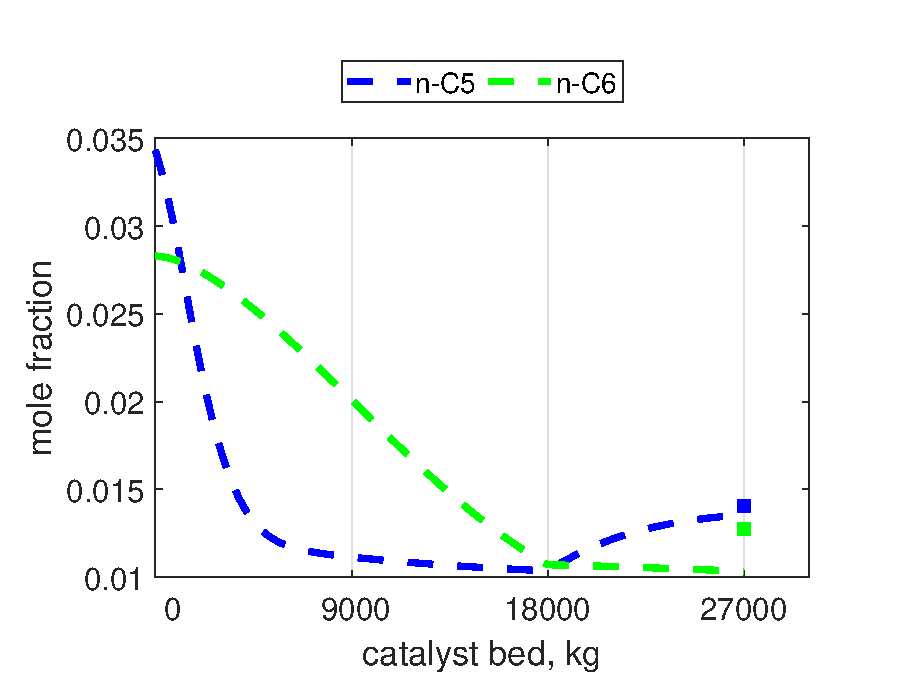
\includegraphics[width=0.9\linewidth]{1.eps} \\ (a)}
\end{minipage}
\begin{minipage}{0.45\linewidth}
\center{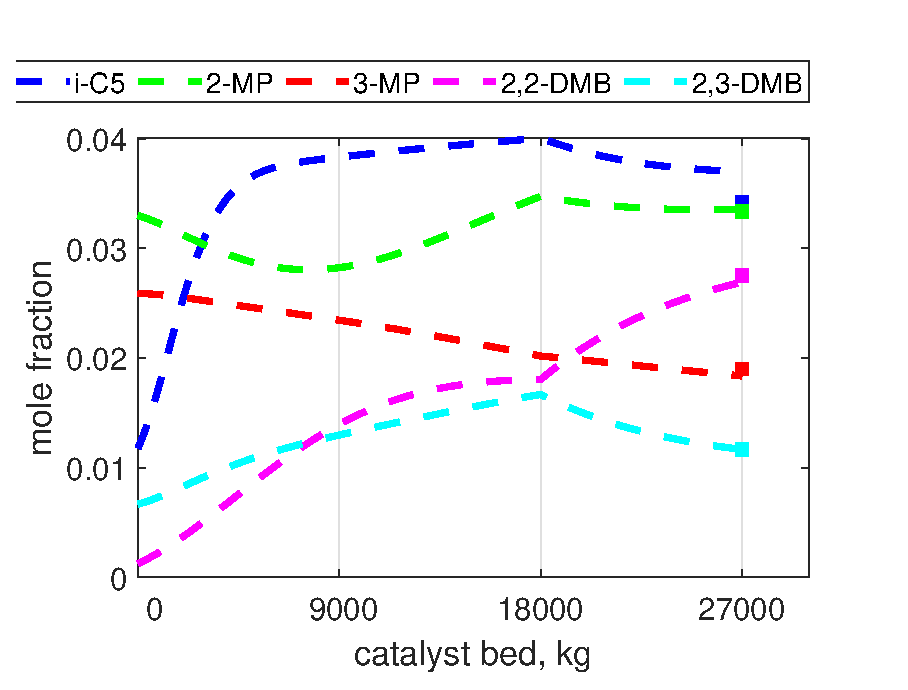
\includegraphics[width=0.9\linewidth]{2.eps} \\ (b)}
\end{minipage}
\caption{Changes in concentrations of (a) $n$-pentane ($n$-C$_5$) and $n$-hexane ($n$-C$_6$), (b) isopentane (i-C5), 2-methylpentane (2-MP), 3-methylpentane (3-MP), 2,2-dimethylbutane(2,2-DMB), 2,3-dimethylbutane (2,3-DMB).}\label{fig:res1}
\end{figure}  

\begin{figure}
\center
\begin{minipage}{0.45\linewidth}
\center{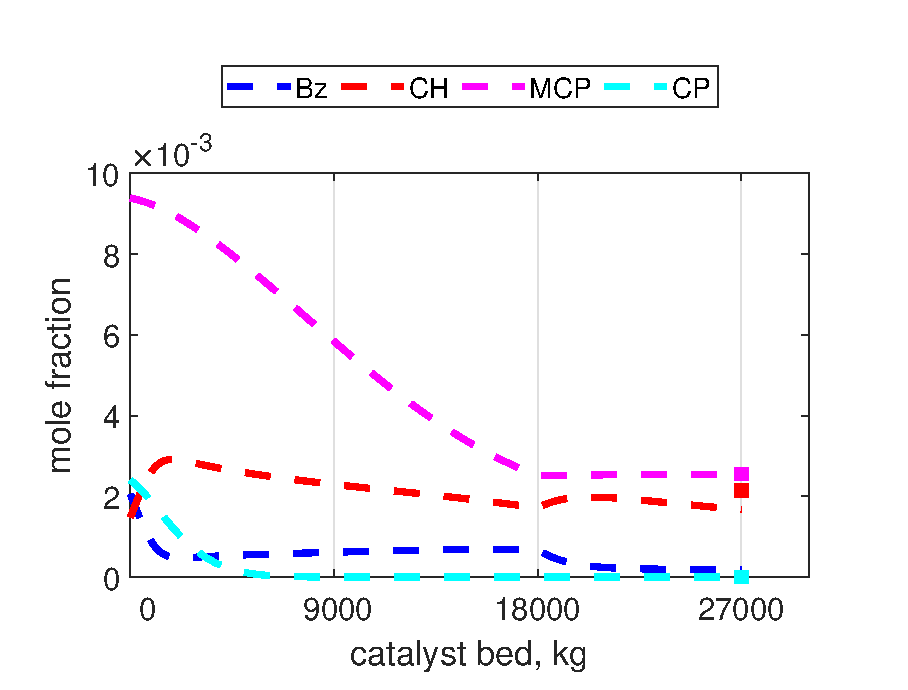
\includegraphics[width=0.9\linewidth]{3.eps} \\ (a)}
\end{minipage}
\begin{minipage}{0.45\linewidth}
\center{\includegraphics[width=0.9\linewidth]{4.eps} \\ (b)}
\end{minipage}
\caption{Changes in (a) concentrations of benzene, cyclohexane (CH*), methyl cyclopentane (MCP), cyclopentane (CP), (b) temperature.}\label{fig:res2}
\end{figure}  

Figure \ref{fig:res1} (a) shows that the concentrations of n-pentane and n-hexane are continuously decreasing. This is mainly due to the transformation of alkanes of normal (linear) structure into the corresponding isomers, which is reflected in Figure \ref{fig:res1} (b). With the transformation of n-pentane, everything is natural, since only one isomer is known. And in the case of n-hexane, everything is somewhat different: first, the conversion of n-hexane is carried out into isomers 2-methylpentane and 3-methylpentane, and the latter are further converted into 2,2-dimethylbutane and 2,3-dimethylbutane.

According to Figure \ref{fig:res2} (a), it can be seen that the concentration of cyclopentane in reactor I gradually decreases to zero.  The decrease in cyclopentane concentration can be explained by the hydrogenation reaction to $n$-pentane. According to Figure \ref{fig:res1} (a), this is probably the reason for the increase in the concentration of $n$-pentane at the beginning of reactor I.
Also, this figure shows a sharp decrease in the concentration of benzene, presumably due to hydrogenation reactions.

Figure \ref{fig:res2} (b) shows a graph of temperature changes in reactors I-III. According to the technological scheme, refrigeration equipment for cooling the reaction mixture is installed after reactor II. A gradual increase in temperature in reactors III here indicates the presence of isomerization reactions that occur with a slight exothermic effect.

It is worth noting that the composition of the products at the outlet of the last reactor and the temperature differences in all reactors are close to industrial data. Thus, these facts may indicate the adequacy of the model we have developed.

%%%%%%%%%%%%%%%%%%%%%%%%%%%%%%%%%%%%%%%%%%

%%%%%%%%%%%%%%%%%%%%%%%%%%%%%%%%%%%%%%%%%%
\vspace{6pt} 

%%%%%%%%%%%%%%%%%%%%%%%%%%%%%%%%%%%%%%%%%%


%%%%%%%%%%%%%%%%%%%%%%%%%%%%%%%%%%%%%%%%%%
\authorcontributions{Conceptualization, K.B. and I.G.; methodology, K.B. and I.G.; software, E.K., I.L. and L.E.; validation, A.F.;  resources, A.F.;  writing---original draft preparation, K.B. and A.F.; writing---review and editing, R.F. and L.E.; visualization, R.F.; supervision, I.G.. All authors have read and agreed to the published version of the manuscript.}

\funding{This research was funded by RFBR, project No.\,19-37-60014 (L.E.; mathematical model), and by the Russian Science Foundation, project No.\,21-11-00204 (K.B, I.L., E.K.; parallel algorithm)}

\institutionalreview{Not applicable.}

\informedconsent{Not applicable.}

\dataavailability{Not applicable.} 
\conflictsofinterest{The authors declare no conflict of interest.} 

\abbreviations{Abbreviations}{
The following abbreviations are used in this manuscript:\\

\noindent 
\begin{tabular}{@{}ll}
2-MP & 2-methylpentane\\
3-MP & 3-methylpentane\\
2,2-DMB  & 2,2-dimethylbutane\\
2,3-DMB & 2,3-dimethylbutane\\
CH* & cyclohexane\\
MCP & methylcyclopentane\\
B & benzene\\
CP & cyclopentane
\end{tabular}
}

%%%%%%%%%%%%%%%%%%%%%%%%%%%%%%%%%%%%%%%%%%
%% Optional
\appendixtitles{no} % Leave argument "no" if all appendix headings stay EMPTY (then no dot is printed after "Appendix A"). If the appendix sections contain a heading then change the argument to "yes".
\appendixstart
\appendix
\section[\appendixname~\thesection]{}
%\subsection[\appendixname~\thesubsection]{}
The table \ref{tab_kinetics} is a numerically calculated kinetic parameters of a chemical reaction.

\begin{table}[H] 
\caption{Kinetic parameters of the catalytic isomerisation reaction of the pentane-hexane fraction, according to the scheme of chemical transformations (Table \ref{tab_chemistry}).\label{tab_kinetics}}
\newcolumntype{C}{>{\centering\arraybackslash}X}
\begin{tabularx}{\textwidth}{CCCCCC}
\toprule
\textbf{No}	& \textbf{$E$, kcal/mol} & \textbf{$\log k_0$} & \textbf{No}	& \textbf{$E$, kcal/mol} & \textbf{$\log k_0$} \\
\midrule
1  & 149.320 & 18.492 & 25 & 141.046 & 5.799 \\
2  & 129.372 & 15.604 & 26 & 80.093 & 4.401 \\
3  & 108.439 & 9.286 & 27 & 177.947 & 3.694 \\
4  & 87.168 & 9.002 & 28 & 92.282 & 10.670  \\
5  & 123.830 & 14.203 & 29 & 159.368 & 16.169 \\
6  & 162.603 & 17.997 & 30 & 97.215 & 9.612 \\
7 & 161.429 & 17.114 & 31 & 188.306 & 7.194  \\
8 & 142.261 & 12.667  & 32 & 111.789 & 11.467 \\
9 & 127.715 & 12.130 & 33 & 124.370 & 12.764 \\
10 & 96.409 & 11.318 & 34 & 101.952 & 6.352 \\
11 & 64.223 & 7.214 & 35 & 131.079 & 16.427  \\
12 & 94.973	& 8.388 & 36 & 177.771 & 11.250  \\
13 & 174.387 & 7.600 & 37 & 72.632 & 15.123 \\
14 & 161.502 & 18.146 & 38 & 67.167 & 14.013 \\
15 & 98.296 & 11.305 & 39 & 230.976 & 12.798 \\
16 & 104.987 & 11.499 & 40 & 214.539 & 13.532  \\
17 & 42.264 & 3.622 & 41 & 291.967 & 26.096  \\
18 & 45.070 & 5.530 & 42 & 185.864 & 20.281 \\
19 & 162.126 & 21.057 & 43 & 134.411 & 14.229 \\
20 & 231.848 & 28.391 & 44 & 82.0120 & 8.262 \\
21 & 245.107 & 28.488 & 45 & 388.331 & 17.056 \\
22 & 204.298 & 23.176 & 46 & 286.722 & 18.898 \\
23 & 53.493 & 5.911 & 47 & 356.242 & 5.148  \\
24 & 252.728 & 1.600 & 48 & 355.642 & 9.141  \\
\bottomrule
\end{tabularx}
\end{table}


%%%%%%%%%%%%%%%%%%%%%%%%%%%%%%%%%%%%%%%%%%
\begin{adjustwidth}{-\extralength}{0cm}
%\printendnotes[custom] % Un-comment to print a list of endnotes

\reftitle{References}

% Please provide either the correct journal abbreviation (e.g. according to the “List of Title Word Abbreviations” http://www.issn.org/services/online-services/access-to-the-ltwa/) or the full name of the journal.
% Citations and References in Supplementary files are permitted provided that they also appear in the reference list here. 

%=====================================
% References, variant A: external bibliography
%=====================================
\bibliography{bibliography.bib}

%=====================================
% References, variant B: internal bibliography
%=====================================
%\begin{thebibliography}{999}

% Reference 1
%\bibitem[Author1(year)]{ref-journal}
%Author~1, T. The title of the cited article. {\em Journal Abbreviation} {\bf 2008}, {\em 10}, 142--149.
% Reference 2
%\bibitem[Author2(year)]{ref-book1}
%Author~2, L. The title of the cited contribution. In {\em The Book Title}; Editor 1, F., Editor 2, A., Eds.; Publishing House: City, Country, 2007; pp. 32--58.
% Reference 3
%\bibitem[Author3(year)]{ref-book2}
%Author 1, A.; Author 2, B. \textit{Book Title}, 3rd ed.; Publisher: Publisher Location, Country, 2008; pp. 154--196.
% Reference 4
%\bibitem[Author4(year)]{ref-unpublish}
%Author 1, A.B.; Author 2, C. Title of Unpublished Work. \textit{Abbreviated Journal Name} year, \textit{phrase indicating stage of publication (submitted; accepted; in press)}.
% Reference 5
%\bibitem[Author5(year)]{ref-communication}
%Author 1, A.B. (University, City, State, Country); Author 2, C. (Institute, City, State, Country). Personal communication, 2012.
% Reference 6
%\bibitem[Author6(year)]{ref-proceeding}
%Author 1, A.B.; Author 2, C.D.; Author 3, E.F. Title of presentation. In Proceedings of the Name of the Conference, Location of Conference, Country, Date of Conference (Day Month Year); Abstract Number (optional), Pagination (optional).
% Reference 7
%\bibitem[Author7(year)]{ref-thesis}
%Author 1, A.B. Title of Thesis. Level of Thesis, Degree-Granting University, Location of University, Date of Completion.
% Reference 8
%\bibitem[Author8(year)]{ref-url}
%Title of Site. Available online: URL (accessed on Day Month Year).
%\end{thebibliography}

% If authors have biography, please use the format below
%\section*{Short Biography of Authors}
%\bio
%{\raisebox{-0.35cm}{\includegraphics[width=3.5cm,height=5.3cm,clip,keepaspectratio]{Definitions/author1.pdf}}}
%{\textbf{Firstname Lastname} Biography of first author}
%
%\bio
%{\raisebox{-0.35cm}{\includegraphics[width=3.5cm,height=5.3cm,clip,keepaspectratio]{Definitions/author2.jpg}}}
%{\textbf{Firstname Lastname} Biography of second author}

% For the MDPI journals use author-date citation, please follow the formatting guidelines on http://www.mdpi.com/authors/references
% To cite two works by the same author: \citeauthor{ref-journal-1a} (\citeyear{ref-journal-1a}, \citeyear{ref-journal-1b}). This produces: Whittaker (1967, 1975)
% To cite two works by the same author with specific pages: \citeauthor{ref-journal-3a} (\citeyear{ref-journal-3a}, p. 328; \citeyear{ref-journal-3b}, p.475). This produces: Wong (1999, p. 328; 2000, p. 475)

%%%%%%%%%%%%%%%%%%%%%%%%%%%%%%%%%%%%%%%%%%
%% for journal Sci
%\reviewreports{\\
%Reviewer 1 comments and authors’ response\\
%Reviewer 2 comments and authors’ response\\
%Reviewer 3 comments and authors’ response
%}
%%%%%%%%%%%%%%%%%%%%%%%%%%%%%%%%%%%%%%%%%%
\end{adjustwidth}
\end{document}

